\begin{filecontents*}{\jobname.xmpdata}
   \Title{Compact Symmetry Breaking for Tournaments}
   \Author{Evan Lohn\sep Chris Lambert\sep Marijn J.H. Heule}
   \Publisher{TU Wien Academic Press}
\end{filecontents*}

\documentclass[year=22,pdfa]{fmcad}
\usepackage{graphicx}
\usepackage{tikz}
\usepackage{pgfplots}
\usepackage{amsmath}
\usepackage{amssymb}
\usepackage{amsthm}
\usepackage{cleveref}
\usepackage{cite}
\usepackage[section]{placeins}

\usetikzlibrary{shapes}

\newcommand{\zero}{\tikz[baseline=(char.base)]{
            \node[fill=white,shape=circle,inner sep=1pt] (char) {\textcolor{black}{0}};}}
\newcommand{\one}{\tikz[baseline=(char.base)]{
            \node[fill=black,shape=circle,inner sep=1pt] (char) {\textcolor{white}{1}};}}
\newcommand{\none}{\tikz[baseline=(char.base)]{
            \node[fill=white,shape=circle,inner sep=1pt] (char) {\textcolor{white}{1}};}}

\usepackage{multirow,bigdelim,blkarray}

\pgfplotsset{width=10cm,compat=1.9}

\newcommand{\N}{\mathbb{N}}

\newcommand\overmat[3][0pt]{%
  \makebox[0pt][l]{$\smash{\overbrace{\phantom{%
    \begin{matrix}\phantom{\rule{0pt}{#1}}#3\end{matrix}}}^{#2}}$}#3}

\usetikzlibrary{arrows}

\def\BibTeX{{\rm B\kern-.05em{\sc i\kern-.025em b}\kern-.08em
    T\kern-.1667em\lower.7ex\hbox{E}\kern-.125emX}}

\begin{document}
\title{Compact Symmetry Breaking for Tournaments}

\author{
\IEEEauthorblockN{Evan Lohn\orcid{0000-0001-7843-6136}}
\IEEEauthorblockA{Carnegie Mellon University, Pittsburgh, United States\\
 \emph{elohn@andrew.cmu.edu}}
 \and
\IEEEauthorblockN{Chris Lambert}
\IEEEauthorblockA{Carnegie Mellon University, Pittsburgh, United States\\
 \emph{chrislambert@cmu.edu}}
\IEEEauthorblockN{Marijn J.H. Heule\orcid{0000-0002-5587-8801}}
\IEEEauthorblockA{Carnegie Mellon University, Pittsburgh, United States\\
 \emph{marijn@cmu.edu}}

}

\maketitle

\begin{abstract}
Isolators are a useful tool for reducing the computation needed to solve graph existence problems via SAT.  We extend techniques for creating isolators for undirected graphs to the tournament (complete, directed) case, noting several parallels in properties of isolators for the two classes. We further present an algorithm for constructing $n$-vertex tournament isolators with $\Theta(n \log n)$ unit clauses. Finally, we show the utility of our new isolators in computations of tournament Ramsey numbers.
\end{abstract}

\begin{IEEEkeywords}
Satisfiability, Symmetry-breaking, Directed-graphs, Tournaments, Isolators.
\end{IEEEkeywords}


\section{Introduction}

In recent years, SAT solvers have been used to solve several difficult combinatorial problems \cite{ref_keller,ref_schur,ref_pythagorean}. However, naive encodings of SAT problems often include undesired symmetries, i.e. certain matching subsets of variables that result in equivalent subproblems when given equivalent assignments. To prove the original formula unsatisfiable, in the worst case a solver must search through all possible symmetric parts of the problem space, which slows the generation of unsatisfiable proofs unnecessarily. Similarly, while the solver tries to find a satisfying assignment, symmetries in the input formula may cause the solver to effectively re-explore the same part of the search space even after proving the lack of a solution in a symmetric part of the problem.

The most common way of reducing the impact of symmetries in a given formula is by adding a set of new clauses called a Symmetry-Breaking Predicate (SBP) to the formula before solving \cite{ref_SBP, ref_SBP2, ref_approxmc}. The goal of a SBP is to preserve the satisfiability of the formula while removing from consideration any regions of the search space known to be symmetric to other regions. In this work we focus on SBP's for \emph{graph existence problems}, which are problems that can be solved by checking if a graph with a particular structure exists. Solving such problems is an active area of research \cite{ref_vdw, ref_ramseyk, ref_5cycle}. A large class of problem symmetries in graph existence problems naturally results from the existence of isomorphic labeled graphs. These symmetries exist independent of any desired graph property related to graph structure. Rather, they occur because SAT solvers must search the space of labeled graphs in order to prove the (non-)existence of an unlabeled graph. A SBP that targets graph isomorphisms is known as an isolator. Isolators that break many symmetries with few clauses are most useful in practice, as SAT solvers generally take longer to solve formulas with more clauses. Such isolators are often described as ``short'', ``small'', or ``compact.''


Prior work has shown that it is possible to generate small isolators for undirected graphs \cite{ref_heule}. The present work instead handles the generation of short isolators for tournaments: complete, directed graphs. There are several mathematically interesting questions one can ask about tournaments that motivate the generation of tournament isolators. For example, Sumner's conjecture and various election models in social choice theory rely on tournament properties \cite{ref_sumner,ref_social_choice}. Tournament isolators can also aid in the search for doubly-regular tournaments. Doubly-regular tournaments are a class of tournaments that (among many other properties) can be efficiently transformed to skew-symmetric Hadamard matrices \cite{ref_hadamard}, which have a wide array of practical uses. However, the most well-known question about tournament structure is the Tournament Ramsey number problem, an analog to Ramsey numbers \cite{ref_ramsey_survey} that asks the question of ``in what size tournament $n$ must a transitive subtournament of size $k$ exist.'' A (sub)tournament is \emph{transitive} if it contains no cycles. Calculating the tournament Ramsey number for $k=7$ is likely the limit of currently known techniques, and doing so would be impactful for the mathematical community.

The first contribution of this work is the generation of compact tournament isolators that asymptotically match the search space reduction of a perfect isolator. Second, we present a methodology for the generation of compact isolators for small tournaments that extends prior work on undirected tournaments \cite{ref_heule}.  Finally, we demonstrate the practical usage of our small isolators for finding larger graphs relevant to the search for tournament Ramsey numbers.


\section{Preliminaries}

We define the following common concepts from SAT literature:
A \emph{literal} is either a variable or a negated variable. We use $\lnot$ to denote negation.
A \emph{clause} is a disjunction of literals.
A \emph{unit clause} (sometimes referred to as simply a \emph{unit}) is a clause containing exactly one literal.
A \emph{Conjunctive Normal Form (CNF) formula} is a conjunction of clauses. Unless otherwise specified, ``formula'' refers to ``CNF formula.''
An \emph{assignment} $\alpha$ is a function from variables to truth values (True/False). $\alpha$ satisfies a formula $F$ if the boolean function denoted by $F$ returns True given the inputs specified by $\alpha$.


We also define several graph-theoretic concepts.
A tournament $G = (V,E)$ is a complete directed graph; more formally, $\forall (v_1, v_2) \in V \times V, v_1 \neq v_2 \rightarrow ((v_1, v_2) \in E) \oplus ((v_2, v_1) \in E)$ and $\forall v \in V, (v,v) \notin E$, where $\oplus$ is the XOR operation. The phrase ``$G$ is an $n$-vertex tournament'' means $|V| = n$.
Given an $n$-vertex tournament $G= (V,E)$ and a permutation $\pi$ on $V$, $\pi(G)$ is defined as $\pi(G) = (V, \{(\pi(v_1), \pi(v_2)) | (v_1, v_2) \in E\}$) and is colloquially referred to as applying $\pi$ to $G$.
Two $n$-vertex tournaments $G_1, G_2$ are \emph{isomorphic} (written $G_1 \simeq G_2$) exactly when there exists a permutation $\pi$ on the vertices of $G_1$ such that $\pi(G_1) = G_2$. When any such $\pi$ exists, it is referred to as an \emph{isomorphism} between $G_1$ and $G_2$.
The \emph{isomorphism class} (also, \emph{equivalence class}) $I_G$ of a tournament $G$ is defined as $I_G = \{G' | G \simeq G'\}$.
An \emph{automorphism} $\pi$ on a tournament $G$ is any permutation $\pi$ such that $\pi(G) = G$. The set of automorphisms of $G$ form a group under function composition. This group is referred to as $Aut(G)$.

\section{Isolator Notation and Concepts}

To search for a tournament $G$ satisfying some structural property, we define variables with the semantics ``edge $e$ exists in graph $G$'' for use in a formula $F$. We say that $F$ \emph{admits} a graph $G'$ exactly when there exists a satisfying assignment to the conjunction of $F$ and the set of unit clauses semantically implied by the edges of $G'$.
An \emph{isolator} for $n$-vertex tournaments is a formula $F$ that admits at least one tournament from each equivalence class on $n$-vertex tournaments.
A \emph{perfect} isolator is an isolator that admits \textit{exactly} one tournament from each equivalence class.
A perfect isolator $F$ is \emph{optimal} if there does not exist a perfect isolator with fewer non-unit clauses than $F$.
A \emph{compact} or \emph{short} isolator is not rigorously defined. Rather, it describes an isolator with few enough non-unit clauses to be of practical use in solving SAT problems.

In this work, vertices will be denoted with lowercase letters $a,b,c, \dots$ or with $v_1, v_2, \dots, v_n$ when an ordering of the vertices is relevant. Arcs (directed edges) will be referred to with $(u,v)$, meaning ``there is an arc from $u$ to $v$.'' In our construction of isolators, each variable is written in the form $uv$ and has the semantics ``arc $(u,v)$ exists in the graph.'' Note that the literal $\lnot uv$ therefore means ``arc $(v,u)$ exists in the graph.'' 


\subsection{Short Isolator Examples}
Consider the following two labeled 3-vertex tournaments.

\noindent

\begin{figure}[h]
\centering
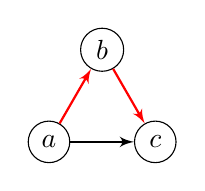
\begin{tikzpicture}[scale=.9]
\tikzset{vertex/.style = {shape=circle,draw,minimum size=1.5em}}
\tikzset{edge/.style = {->,> = latex'}}
% vertices
\node[vertex] (a) at  (-.75,0) {$\!a\!$};
\node[vertex] (b) at  (0,1.3) {$\!b\!$};
\node[vertex] (c) at  (.75,0) {$\!c\!$};

%edges
\draw[edge, thick][red] (a) to (b);
\draw[edge, thick] (a) to (c);
\draw[edge, thick][red] (b) to (c);

\end{tikzpicture}
~~~~~~~~
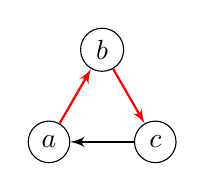
\begin{tikzpicture}[scale=.9]
\tikzset{vertex/.style = {shape=circle,draw,minimum size=1.5em}}
\tikzset{edge/.style = {->,> = latex'}}

\node[vertex] (a) at  (-.75,0) {$\!a\!$};
\node[vertex] (b) at  (0,1.3) {$\!b\!$};
\node[vertex] (c) at  (.75,0) {$\!c\!$};

%edges
\draw[edge, thick][red] (a) to (b);
\draw[edge, thick] (c) to (a);
\draw[edge, thick][red] (b) to (c);

\end{tikzpicture}
\end{figure}

These tournaments represent the only two equivalence classes for $n=3$ tournaments: a cycle and a transitive tournament. While any combination of a cycle and transitive tournament would suffice to represent both equivalence classes, the tournaments chosen above have the interesting property of sharing two edges $ab$ and $bc$ (colored red). This property allows us to produce a short formula that admits both graphs:
\[
ab \land bc.
\]

This formula admits exactly one of the two labeled cycles and one of the six labeled transitive tournaments on 3 vertices, and does so with the fewest possible clauses. Therefore, $ab \land bc$ is a perfect, optimal isolator for $n=3$ tournaments.

Figure \ref{iso4} displays canonical representatives of all 4 isomorphism classes for $n=4$ tournaments. We note that once again all highlighted edges have the same edge labels across graphs, and all permutations of non-highlighted edges are present. So, a short formula that admits exactly the set of graphs in the figure is
\[
ab \land bc \land cd \land ad.
\]

While the optimal isolators for $n=3,4$ are comprised entirely of unit clauses, this pattern does not hold for $n=5$. Table \ref{tab:smallest_isolators_found} contains the number of unit and non-unit clauses for our isolators on $n \le 8$ vertices.


\begin{figure}[t]
\centering
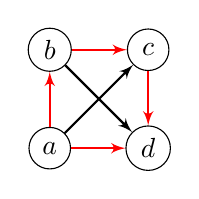
\begin{tikzpicture}
\tikzset{vertex/.style = {shape=circle,draw,minimum size=1.5em}}
\tikzset{edge/.style = {->,> = latex'}}
\node[vertex] (a) at (0,0) {$\!a\!$};
\node[vertex] (b) at (0,1.25) {$\!b\!$};
\node[vertex] (c) at (1.25,1.25) {$\!c\!$};
\node[vertex] (d) at (1.25,0) {$\!d\!$};

\draw[edge, thick][red] (a) to (b);
\draw[edge, thick] (a) to (c);
\draw[edge, thick][red] (b) to (c);
\draw[edge, thick][red] (c) to (d);
\draw[edge, thick] (b) to (d);
\draw[edge, thick][red] (a) to (d);
\end{tikzpicture}
~~
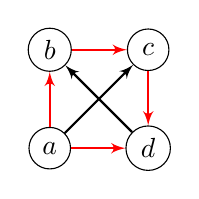
\begin{tikzpicture}
\tikzset{vertex/.style = {shape=circle,draw,minimum size=1.5em}}
\tikzset{edge/.style = {->,> = latex'}}
\node[vertex] (a) at (0,0) {$\!a\!$};
\node[vertex] (b) at (0,1.25) {$\!b\!$};
\node[vertex] (c) at (1.25,1.25) {$\!c\!$};
\node[vertex] (d) at (1.25,0) {$\!d\!$};

\draw[edge, thick][red] (a) to (b);
\draw[edge, thick] (a) to (c);
\draw[edge, thick][red] (b) to (c);
\draw[edge, thick][red] (c) to (d);
\draw[edge, thick] (d) to (b);
\draw[edge, thick][red] (a) to (d);
\end{tikzpicture}
~~
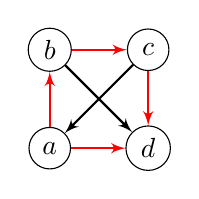
\begin{tikzpicture}
\tikzset{vertex/.style = {shape=circle,draw,minimum size=1.5em}}
\tikzset{edge/.style = {->,> = latex'}}
\node[vertex] (a) at (0,0) {$\!a\!$};
\node[vertex] (b) at (0,1.25) {$\!b\!$};
\node[vertex] (c) at (1.25,1.25) {$\!c\!$};
\node[vertex] (d) at (1.25,0) {$\!d\!$};

\draw[edge, thick][red] (a) to (b);
\draw[edge, thick] (c) to (a);
\draw[edge, thick][red] (b) to (c);
\draw[edge, thick][red] (c) to (d);
\draw[edge, thick] (b) to (d);
\draw[edge, thick][red] (a) to (d);
\end{tikzpicture}
~~
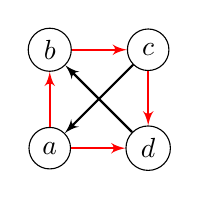
\begin{tikzpicture}
\tikzset{vertex/.style = {shape=circle,draw,minimum size=1.5em}}
\tikzset{edge/.style = {->,> = latex'}}
\node[vertex] (a) at (0,0) {$\!a\!$};
\node[vertex] (b) at (0,1.25) {$\!b\!$};
\node[vertex] (c) at (1.25,1.25) {$\!c\!$};
\node[vertex] (d) at (1.25,0) {$\!d\!$};

\draw[edge, thick][red] (a) to (b);
\draw[edge, thick] (c) to (a);
\draw[edge, thick][red] (b) to (c);
\draw[edge, thick][red] (c) to (d);
\draw[edge, thick] (d) to (b);
\draw[edge, thick][red] (a) to (d);
\end{tikzpicture}

\caption{All isomorphism class representatives admitted by a perfect, optimal isolator for 4-vertex tournaments. Red edges are edges fixed by unit clauses of the isolator, and the isolator has only unit clauses.} 
\label{iso4}
\end{figure}

\subsection{Comparison of undirected graph and tournament isolators}

Although the majority of this work focuses on tournament isolators, there are many interesting parallels between undirected and tournament isolators. In an undirected context, the \emph{existence} of edge $(u,v)$ is denoted by the literal $uv$, while its nonexistence is denoted by the literal's negation $\lnot uv$.
Because edgeless and complete graphs are isomorphism classes for any $n$ in the undirected case, every clause of an undirected graph isolator containing only arc literals must contain at least one positive and one negative literal. These two graphs do not exist in the case of tournaments; the closest parallel is transitive tournaments. Unlike the set of $n$-vertex undirected graphs which contains exactly one empty graph and one complete graph with $n!$ automorphisms each, there are $n!$ isomorphic transitive tournaments on $n$ vertices. It is possible to select the particular transitive tournament $TT$ that an isolator admits by ensuring that at least one edge from $TT$ is present in each clause of the isolator. A simple way to do so is ensure each clause contains at least one edge $uv$ s.t. $u<v$ in vertex numbering. 

One consequence of undirected isolators requiring at least one positive and one negative literal per clause is that undirected isolators have no unit clauses. However, while negating all literals in an undirected isolator produces another undirected isolator (because the existence and non-existence of an edge is symmetric), there is no direct parallel to be found in tournaments as edge directionality does not have this property.

Another interesting difference between undirected graphs and tournaments is the low number of isomorphism classes for tournaments when $n$ is small (see table \ref{tab:smallest_isolators_found}). Intuitively, this happens because it is ``easier'' for tournaments to be isomorphic. The two options for the edge between vertices $u$ and $v$ in the undirected case are $uv$ existing or not existing. Crucially, an undirected graph $G$ will never be isomorphic to $G'$ constructed by adding or removing an edge of $G$, which is an operation that can be seen as ``flipping'' an edge to its other possibility. However, ``flipping'' an edge of a tournament $T$ by changing the edge's direction will produce $T' \simeq T$ iff the two vertices $u$ and $v$ of the flipped edge had the same edges to the rest of the graph (the isomorphism is via the permutation that swaps $u$ and $v$). Although this discrepancy exists for small $n$, the numbers of isomorphism classes for undirected graphs and tournaments are remarkably close for larger $n$ (see OEIS A000088, A00056 \cite{ref_oeis}). Therefore, we expect that perfect, optimal isolators for undirected graphs and tournaments will have similar numbers of clauses for larger $n$.


\subsection{Arc Literal Numbering}
Each $uv$ must be assigned a corresponding integer to conform to the commonly used DIMACS CNF format.
To do so, we specify a function $idx_n(u,v)$ to map each possible arc $(u,v)$ in an $n$-vertex tournament to a unique integer identifier.  Because exactly one of $(u,v)$ and $(v,u)$ must exist for any two vertices $u,v$, $\mathit{idx}$ must satisfy $\mathit{idx}_n(u,v) = -\mathit{idx}_n(v,u)$. To facilitate isolator comparisons across different $n$, $\mathit{idx}$ also should satisfy the property that $\mathit{idx}_n(u,v) = \mathit{idx}_{n+1}(u,v)$. We therefore drop the subscript $n$ when referring to $\mathit{idx}_n(u,v) $ in the future, as its value does not depend on $n$. 

In particular, $\mathit{idx}$ is inductively defined as follows for an $n+1$-vertex tournament with vertices $v_1, v_2,,...v_n, v_{n+1}$. Let $K = n(n-1)/2$ be the largest output of $\mathit{idx}$ for an $n$-vertex tournament (implying base case $\mathit{idx}(v_1,v_2) = 1$ when $n=2$). Applying $\mathit{idx}$ to each of the arcs $(v_1,v_{n+1}), (v_2,v_{n+1}), ... (v_n, v_{n+1})$ yields $K+1, K+2,...,K+n$, respectively. All arcs not included in this definition are of the form $(v_w, v_u)$ where $w>u$, and are defined by the earlier mentioned constraint of $\mathit{idx}(u,v) = -\mathit{idx}(v,u)$.


\section{Unit Clauses}

In practice, SAT solvers immediately reduce formulas with unit clauses to shorter formulas without units via unit propagation. Additionally, each unit clause reduces the size of the search space by a factor of 2. Therefore, it is practically useful to create isolators with as many units as possible. The following sections detail and analyze our various methods for creating isolators with many unit clauses.

\subsection{Provable Units}
While constructing smaller isolators using the techniques above, we opted to manually inspect our results and see what patterns they shared.  In doing so, we rediscovered a well-known fact from graph theory literature; every tournament contains a Hamiltonian path \cite{ref_tournament_book}. Proof sketch: inductively consider a length $n$ Hamiltonian path $v_1, v_2, ... v_n$ in an $n+1$-vertex tournament $G=(V,E)$. For the vertex $v_{n+1}$ not part of the path, in the case that either $(v_{n+1}, v_1)$ or $(v_n, v_{n+1})$ is in $E$, a length $n+1$ Hamiltonian path is formed. Otherwise, $(v_1, v_{n+1})$ and $(v_{n+1}, v_{n})$ are in $E$ and thus there must exist consecutive vertices $v_i,v_{i+1}$ in the Hamiltonian path such that arcs $(v_i,v_{n+1})$ and $(v_{n+1},v_{i+1})$ are in $E$. In this case, the sequence $v_1,v_2,...v_i, v_{n+1}, v_{i+1},...v_n$ forms a length $n+1$ Hamiltonian path. As a result of this property, a set of unit clauses describing a Hamiltonian path on an $n$-vertex tournament is always a valid $n$-vertex isolator.


Given the utility of unit clauses in isolators, it is natural to ask how many units there can possibly be in an $n$-vertex isolator. As it turns out, there is a long-known result from graph theory that implies that asymptotically there are at most $O(n\log n)$ units possible. By the orbit-stabilizer theorem, the size of the equivalence class of a graph $G$ on $n$ vertices is $\frac{n!}{|Aut(G)|}$, where $Aut(G)$ is the set of distinct automorphisms of $G$. In 1963 Erd\H{o}s and R{\'e}nyi proved that as $n$ approaches infinity, the proportion of undirected graphs of size $n$ with with nontrivial automorphisms approaches 0 \cite{ref_asymmetric}. The same result for tournaments directly follows. Therefore, a proportion of tournaments approaching 1 has equivalence classes of size $n!$, so the asymptotic number of equivalence classes is
\[
\frac{2^{n \choose 2}}{n!} \in \Theta(\frac{2^{n \choose 2}}{2^{n\log n}}) = \Theta(2^{{n \choose 2} - n\log n}).
\]

An isolator with $k$ unit clauses for $n$-vertex graphs admits at most $2^{{n \choose 2} - k}$ equivalence class representatives, so in order to admit at least one member of each equivalence class (by the definition of an isolator), the number of units in an isolator must also be asymptotically upper-bounded by $n \log n$.

In the next section, we provide a procedure that achieves this bound.

\subsection{TT-fixing}


In situations where we know that every member of the class of $n$-vertex tournaments contains a $TT_k$ (a transitive tournament of size k), we also know that every equivalence class must contain a member with the tournament fixed in some arbitrary position and orientation (i.e. vertices $1$ through $k$ in ascending order). Therefore, any formula that \emph{fixes} (i.e. asserts the existence of) a $TT_k$ on the class of $n$-vertex tournaments is a valid isolator. Because the remaining subset of $n-k$ non-fixed vertices also forms a tournament, further knowledge about the existence of a transitive tournament within the remaining $n-k$ vertices can be used to fix (via units) another transitive tournament within the $n-k$ vertex subtournament. This procedure can be repeated until all vertices of the original tournament are part of some fixed transitive subtournament. Tournament Ramsey numbers provide exactly the required information about the existence of a transitive subtournament. In fact, tournament Ramsey numbers $R(k)$ (when known) provide the \textit{largest} $TT_k$ guaranteed to exist in a tournament of size at least $R(k)$. Therefore, tournament Ramsey numbers (as well as upper bounds, which exist for arbitrarily large $n$) can be used to iteratively construct large sets of unit clauses for tournament isolators: we will refer to this process as TT-fixing.

TT-fixing is best understood via a small example like figure \ref{fig:TTfix}. For an arbitrary $16$-vertex tournament $G$, $R(5) = 14$ implies that $G$ must contain a $TT_5$ as a subtournament. Therefore, the arcs between vertices $v_1 ... v_5$ can be ``fixed'' to be a transitive tournament by generating all unit clauses corresponding to those arcs. However, the remaining $16-5=11$ vertices of $G$ also form an arbitrary subtournament $G'$ on $11$ vertices. Because $R(4) = 8$, a $TT_4$ is guaranteed to exist in $G'$, so we can add unit clauses corresponding to the specific location of that $TT_4$'s existence in vertices $v_6 ... v_9$. The repetition of this procedure down to 1 or 0 remaining vertices is TT-fixing.


\begin{figure}
$$\left[
\begin{array}{c@{\,}c@{\,}c@{\,}c@{\,}c@{\,}c@{\,}c@{\,}c@{\,}c@{\,}c@{\,}c@{\,}c@{\,}c@{\,}c@{\,}c@{\,}c}
\zero & \one & \one & \one & \one & \none & \none & \none & \none & \none & \none & \none & \none & \none & \none & \none\\
\zero & \zero & \one & \one & \one & \none & \none & \none & \none & \none & \none & \none & \none & \none & \none & \none\\
\zero & \zero & \zero & \one & \one & \none & \none & \none & \none & \none & \none & \none & \none & \none & \none & \none\\
\zero & \zero & \zero & \zero & \one & \none & \none & \none & \none & \none & \none & \none & \none & \none & \none & \none\\
\zero & \zero & \zero & \zero & \zero & \none & \none & \none & \none & \none & \none & \none & \none & \none & \none & \none\\
\none & \none & \none & \none & \none & \zero & \one & \one & \one & \none & \none & \none & \none & \none & \none & \none\\
\none & \none & \none & \none & \none & \zero & \zero & \one & \one & \none & \none & \none & \none & \none & \none & \none\\
\none & \none & \none & \none & \none & \zero & \zero & \zero & \one & \none & \none & \none & \none & \none & \none & \none\\
\none & \none & \none & \none & \none & \zero & \zero & \zero & \zero & \none & \none & \none & \none & \none & \none & \none\\
\none & \none & \none & \none & \none & \none & \none & \none & \none & \zero & \one & \one & \none & \none & \none & \none\\
\none & \none & \none & \none & \none & \none & \none & \none & \none & \zero & \zero & \one & \none & \none & \none & \none\\
\none & \none & \none & \none & \none & \none & \none & \none & \none & \zero & \zero & \zero & \none & \none & \none & \none\\
\none & \none & \none & \none & \none & \none & \none & \none & \none & \none & \none & \none & \zero & \one & \one & \none\\
\none & \none & \none & \none & \none & \none & \none & \none & \none & \none & \none & \none & \zero & \zero & \one & \none\\
\none & \none & \none & \none & \none & \none & \none & \none & \none & \none & \none & \none & \zero & \zero & \zero & \none\\
\none & \none & \none & \none & \none & \none & \none & \none & \none & \none & \none & \none & \none & \none & \none & \zero\\
\end{array}
\right]$$

\caption{A visual depiction of the unit clauses provided TT-fixing in the adjacency matrix of an $n=16$ tournament. For entries with value $1$ at row $i$ and column $j$, the unit clause corresponding to $(v_i, v_j)$  is added by TT-fixing. Equivalently, the $1$'s and $0$'s shown will exist in the adjacency matrix of any graph admitted by a TT-fixing isolator. }
\label{fig:TTfix}
\end{figure}


\subsection{TT-fixing gives $\Theta(n\log n)$ units}
Let $units(n)$ be the function that returns the number of units that can be added to an isolator when using the TT-fixing method on $n$-vertex tournaments. Our goal is to prove a lower bound on $units(n)$. Unfortunately, exact tournament Ramsey numbers are non-trivial to calculate (only up to $R(6) = 28$ is known). However, from Erd\H{o}s and Moser  we have that $R(k) \leq 2^{k-1}$ \cite{ref_erdos_ramsey_bounds}, i.e. that a $TT_{k}$ must exist when considering any tournament on $2^{k-1}$ or more vertices. Erd\H{o}s and Moser's bound can thus be used with TT-fixing to lower-bound $units(n)$.

We claim that $units(n) \geq \sum\limits_{i=1}^n \frac{1}{2} \lfloor \log_2(i) \rfloor$. We proceed via induction, with step $n$ depending on step $n-k$, with $k=\lfloor \log_2(n)\rfloor + 1$. The proposition is true for $n=1$ because $0 \geq 0$, $n=2$ because $ 1 \geq 0.5$.  By definition of TT-fixing, for a graph with $n$ vertices we have 

\begin{equation}\label{unitsndef}
units(n) = \frac{k(k-1)}{2}  + units(n-k).
\end{equation} 

By the inductive hypothesis,

 \begin{equation}\label{unitsIH}
 units(n-k) \geq \sum\limits_{i=1}^{n-k} \lfloor \log_2(i)\rfloor/2.
 \end{equation}
 
 Next, we have that 
 \begin{align}
  k\frac{k-1}{2} &= k \lfloor \log_2(n)\rfloor/2 \nonumber \\
   &= \sum\limits_{i=n-k+1}^{n} \lfloor \log_2(n)\rfloor/2 \nonumber \\
  &\geq \sum\limits_{i=n-k+1}^{n} \lfloor \log_2(i)\rfloor/2  \label{unitsk}.
 \end{align}
 
 Combining lower bounds (\ref{unitsIH}) and (\ref{unitsk}) for the terms of \cref{unitsndef} completes the proof: 
 \begin{align}
 units(n) &= \frac{k(k-1)}{2} + units(n-k) \nonumber \\
 &\geq \sum\limits_{i=n-k+1}^{n} \lfloor \log_2(i)\rfloor/2 + \sum\limits_{i=1}^{n-k} \lfloor \log_2(i)\rfloor/2 \\
 &= \sum\limits_{i=1}^{n} \lfloor \log_2(i)\rfloor/2.
 \end{align}
 
 This inequality result directly implies the asymptotic $n\log n$ bound, because $\log_2(n!) \in \Theta(n \log n)$. 

\begin{figure}
\centering
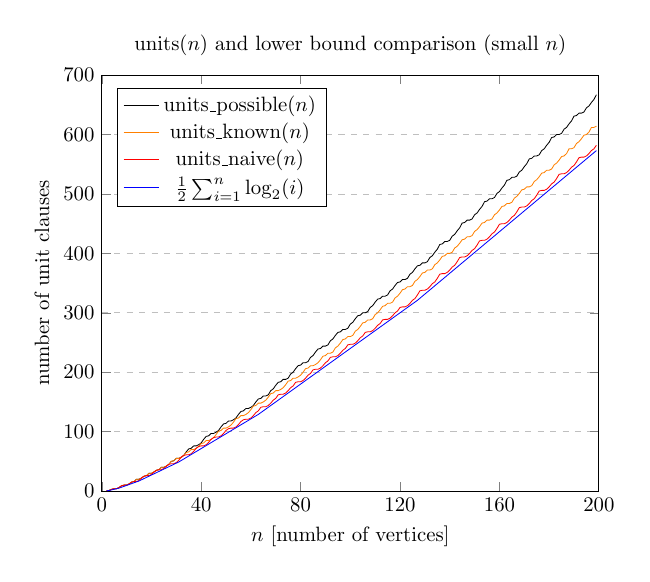
\begin{tikzpicture}[scale = 0.75]
\begin{axis}[
    title={units($n$) and lower bound comparison (small $n$)},
    xlabel={$n$ [number of vertices]},
    ylabel={number of unit clauses},
    xmin=0, xmax=200,
    ymin=0, ymax=700,
    xtick={0,40,80,120,160,200},
    ytick={0,100,200,300,400,500,600,700},
    legend pos=north west,
    ymajorgrids=true,
    grid style=dashed,
]

\addplot[
    color=black,
    ]
    coordinates {
(2,1)(3,1)(4,3)(5,4)(6,4)(7,6)(8,9)(9,10)(10,10)(11,12)(12,15)(13,16)(14,20)(15,20)(16,22)(17,25)(18,26)(19,30)(20,30)(21,32)(22,35)(23,36)(24,40)(25,40)(26,42)(27,45)(28,50)(29,51)(30,55)(31,55)(32,57)(33,60)(34,66)(35,71)(36,72)(37,76)(38,76)(39,78)(40,81)(41,87)(42,92)(43,93)(44,97)(45,97)(46,99)(47,102)(48,108)(49,113)(50,114)(51,118)(52,118)(53,120)(54,123)(55,129)(56,134)(57,135)(58,139)(59,139)(60,141)(61,144)(62,150)(63,155)(64,156)(65,160)(66,160)(67,162)(68,169)(69,172)(70,178)(71,183)(72,184)(73,188)(74,188)(75,190)(76,197)(77,200)(78,206)(79,211)(80,212)(81,216)(82,216)(83,218)(84,225)(85,228)(86,234)(87,239)(88,240)(89,244)(90,244)(91,246)(92,253)(93,256)(94,262)(95,267)(96,268)(97,272)(98,272)(99,274)(100,281)(101,284)(102,290)(103,295)(104,296)(105,300)(106,300)(107,302)(108,309)(109,312)(110,318)(111,323)(112,324)(113,328)(114,328)(115,330)(116,337)(117,340)(118,346)(119,351)(120,352)(121,356)(122,356)(123,358)(124,365)(125,368)(126,374)(127,379)(128,380)(129,384)(130,384)(131,386)(132,393)(133,396)(134,402)(135,407)(136,415)(137,416)(138,420)(139,420)(140,422)(141,429)(142,432)(143,438)(144,443)(145,451)(146,452)(147,456)(148,456)(149,458)(150,465)(151,468)(152,474)(153,479)(154,487)(155,488)(156,492)(157,492)(158,494)(159,501)(160,504)(161,510)(162,515)(163,523)(164,524)(165,528)(166,528)(167,530)(168,537)(169,540)(170,546)(171,551)(172,559)(173,560)(174,564)(175,564)(176,566)(177,573)(178,576)(179,582)(180,587)(181,595)(182,596)(183,600)(184,600)(185,602)(186,609)(187,612)(188,618)(189,623)(190,631)(191,632)(192,636)(193,636)(194,638)(195,645)(196,648)(197,654)(198,659)(199,667)
    };
    \addlegendentry{units\_possible($n$)}

\addplot[
    color=orange,
    ]
    coordinates {
(2,1)(3,1)(4,3)(5,4)(6,4)(7,6)(8,9)(9,10)(10,10)(11,12)(12,15)(13,16)(14,20)(15,20)(16,22)(17,25)(18,26)(19,30)(20,30)(21,32)(22,35)(23,36)(24,40)(25,40)(26,42)(27,45)(28,50)(29,51)(30,55)(31,55)(32,57)(33,60)(34,65)(35,66)(36,70)(37,70)(38,72)(39,75)(40,80)(41,81)(42,85)(43,85)(44,87)(45,90)(46,95)(47,101)(48,102)(49,106)(50,106)(51,108)(52,111)(53,116)(54,122)(55,123)(56,127)(57,127)(58,129)(59,132)(60,137)(61,143)(62,144)(63,148)(64,148)(65,150)(66,153)(67,158)(68,164)(69,165)(70,169)(71,169)(72,171)(73,174)(74,179)(75,185)(76,186)(77,190)(78,190)(79,192)(80,195)(81,200)(82,206)(83,207)(84,211)(85,211)(86,213)(87,216)(88,221)(89,227)(90,228)(91,232)(92,232)(93,234)(94,241)(95,244)(96,249)(97,255)(98,256)(99,260)(100,260)(101,262)(102,269)(103,272)(104,277)(105,283)(106,284)(107,288)(108,288)(109,290)(110,297)(111,300)(112,305)(113,311)(114,312)(115,316)(116,316)(117,318)(118,325)(119,328)(120,333)(121,339)(122,340)(123,344)(124,344)(125,346)(126,353)(127,356)(128,361)(129,367)(130,368)(131,372)(132,372)(133,374)(134,381)(135,384)(136,389)(137,395)(138,396)(139,400)(140,400)(141,402)(142,409)(143,412)(144,417)(145,423)(146,424)(147,428)(148,428)(149,430)(150,437)(151,440)(152,445)(153,451)(154,452)(155,456)(156,456)(157,458)(158,465)(159,468)(160,473)(161,479)(162,480)(163,484)(164,484)(165,486)(166,493)(167,496)(168,501)(169,507)(170,508)(171,512)(172,512)(173,514)(174,521)(175,524)(176,529)(177,535)(178,536)(179,540)(180,540)(181,542)(182,549)(183,552)(184,557)(185,563)(186,564)(187,568)(188,576)(189,576)(190,578)(191,585)(192,588)(193,593)(194,599)(195,600)(196,604)(197,612)(198,612)(199,614)
    };
    \addlegendentry{units\_known($n$)}

\addplot[
    color=red,
    ]
    coordinates {
(2,1)(3,1)(4,3)(5,4)(6,4)(7,6)(8,9)(9,10)(10,10)(11,12)(12,15)(13,16)(14,16)(15,18)(16,22)(17,25)(18,26)(19,26)(20,28)(21,32)(22,35)(23,36)(24,36)(25,38)(26,42)(27,45)(28,46)(29,46)(30,48)(31,52)(32,57)(33,60)(34,61)(35,61)(36,63)(37,67)(38,72)(39,75)(40,76)(41,76)(42,78)(43,82)(44,87)(45,90)(46,91)(47,91)(48,93)(49,97)(50,102)(51,105)(52,106)(53,106)(54,108)(55,112)(56,117)(57,120)(58,121)(59,121)(60,123)(61,127)(62,132)(63,135)(64,141)(65,142)(66,142)(67,144)(68,148)(69,153)(70,156)(71,162)(72,163)(73,163)(74,165)(75,169)(76,174)(77,177)(78,183)(79,184)(80,184)(81,186)(82,190)(83,195)(84,198)(85,204)(86,205)(87,205)(88,207)(89,211)(90,216)(91,219)(92,225)(93,226)(94,226)(95,228)(96,232)(97,237)(98,240)(99,246)(100,247)(101,247)(102,249)(103,253)(104,258)(105,261)(106,267)(107,268)(108,268)(109,270)(110,274)(111,279)(112,282)(113,288)(114,289)(115,289)(116,291)(117,295)(118,300)(119,303)(120,309)(121,310)(122,310)(123,312)(124,316)(125,321)(126,324)(127,330)(128,337)(129,338)(130,338)(131,340)(132,344)(133,349)(134,352)(135,358)(136,365)(137,366)(138,366)(139,368)(140,372)(141,377)(142,380)(143,386)(144,393)(145,394)(146,394)(147,396)(148,400)(149,405)(150,408)(151,414)(152,421)(153,422)(154,422)(155,424)(156,428)(157,433)(158,436)(159,442)(160,449)(161,450)(162,450)(163,452)(164,456)(165,461)(166,464)(167,470)(168,477)(169,478)(170,478)(171,480)(172,484)(173,489)(174,492)(175,498)(176,505)(177,506)(178,506)(179,508)(180,512)(181,517)(182,520)(183,526)(184,533)(185,534)(186,534)(187,536)(188,540)(189,545)(190,548)(191,554)(192,561)(193,562)(194,562)(195,564)(196,568)(197,573)(198,576)(199,582)
    };
    \addlegendentry{units\_naive($n$)}

\addplot[
    color=blue,
    ]
    coordinates {
    (2,0.5)(3,1.0)(4,2.0)(5,3.0)(6,4.0)(7,5.0)(8,6.5)(9,8.0)(10,9.5)(11,11.0)(12,12.5)(13,14.0)(14,15.5)(15,17.0)(16,19.0)(17,21.0)(18,23.0)(19,25.0)(20,27.0)(21,29.0)(22,31.0)(23,33.0)(24,35.0)(25,37.0)(26,39.0)(27,41.0)(28,43.0)(29,45.0)(30,47.0)(31,49.0)(32,51.5)(33,54.0)(34,56.5)(35,59.0)(36,61.5)(37,64.0)(38,66.5)(39,69.0)(40,71.5)(41,74.0)(42,76.5)(43,79.0)(44,81.5)(45,84.0)(46,86.5)(47,89.0)(48,91.5)(49,94.0)(50,96.5)(51,99.0)(52,101.5)(53,104.0)(54,106.5)(55,109.0)(56,111.5)(57,114.0)(58,116.5)(59,119.0)(60,121.5)(61,124.0)(62,126.5)(63,129.0)(64,132.0)(65,135.0)(66,138.0)(67,141.0)(68,144.0)(69,147.0)(70,150.0)(71,153.0)(72,156.0)(73,159.0)(74,162.0)(75,165.0)(76,168.0)(77,171.0)(78,174.0)(79,177.0)(80,180.0)(81,183.0)(82,186.0)(83,189.0)(84,192.0)(85,195.0)(86,198.0)(87,201.0)(88,204.0)(89,207.0)(90,210.0)(91,213.0)(92,216.0)(93,219.0)(94,222.0)(95,225.0)(96,228.0)(97,231.0)(98,234.0)(99,237.0)(100,240.0)(101,243.0)(102,246.0)(103,249.0)(104,252.0)(105,255.0)(106,258.0)(107,261.0)(108,264.0)(109,267.0)(110,270.0)(111,273.0)(112,276.0)(113,279.0)(114,282.0)(115,285.0)(116,288.0)(117,291.0)(118,294.0)(119,297.0)(120,300.0)(121,303.0)(122,306.0)(123,309.0)(124,312.0)(125,315.0)(126,318.0)(127,321.0)(128,324.5)(129,328.0)(130,331.5)(131,335.0)(132,338.5)(133,342.0)(134,345.5)(135,349.0)(136,352.5)(137,356.0)(138,359.5)(139,363.0)(140,366.5)(141,370.0)(142,373.5)(143,377.0)(144,380.5)(145,384.0)(146,387.5)(147,391.0)(148,394.5)(149,398.0)(150,401.5)(151,405.0)(152,408.5)(153,412.0)(154,415.5)(155,419.0)(156,422.5)(157,426.0)(158,429.5)(159,433.0)(160,436.5)(161,440.0)(162,443.5)(163,447.0)(164,450.5)(165,454.0)(166,457.5)(167,461.0)(168,464.5)(169,468.0)(170,471.5)(171,475.0)(172,478.5)(173,482.0)(174,485.5)(175,489.0)(176,492.5)(177,496.0)(178,499.5)(179,503.0)(180,506.5)(181,510.0)(182,513.5)(183,517.0)(184,520.5)(185,524.0)(186,527.5)(187,531.0)(188,534.5)(189,538.0)(190,541.5)(191,545.0)(192,548.5)(193,552.0)(194,555.5)(195,559.0)(196,562.5)(197,566.0)(198,569.5)(199,573.0)
    };
    \addlegendentry{$\frac{1}{2}\sum_{i=1}^n \log_2(i)$}
    
\end{axis}
\end{tikzpicture}
\caption{A visual depiction of how the number of unit clauses produced by TT-fixing grows under different assumptions about Ramsey numbers.} 
\label{pracunits}
\end{figure}

\begin{figure}
\centering
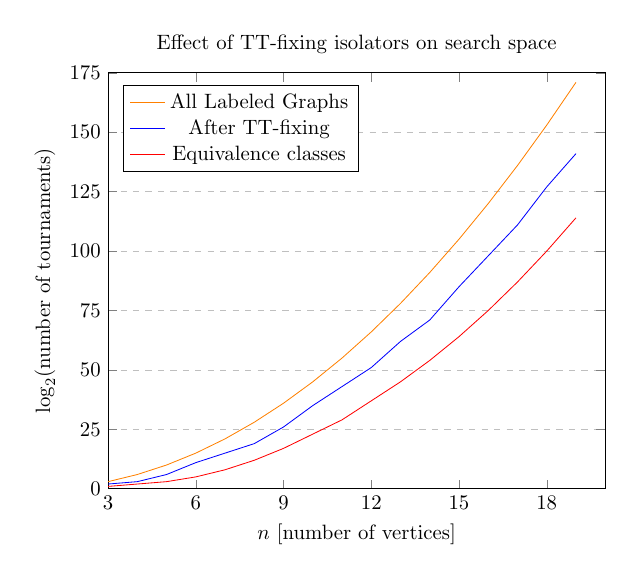
\begin{tikzpicture}[scale=0.75]
\begin{axis}[
    title={Effect of TT-fixing isolators on search space},
    xlabel={$n$ [number of vertices]},
    ylabel={$\log_2$(number of tournaments)},
    xmin=3, xmax=20,
    ymin=0, ymax=175,
    xtick={3,6,9,12,15,18},
    ytick={0,25,50,75,100,125,150, 175},
    legend pos=north west,
    ymajorgrids=true,
    grid style=dashed,
]

\addplot[
    color=orange,
    ]
    coordinates {
(3,3)(4,6)(5,10)(6,15)(7,21)(8,28)(9,36)(10,45)(11,55)(12,66)(13,78)(14,91)(15,105)(16,120)(17,136)(18,153)(19,171)
    };
    \addlegendentry{All Labeled Graphs}

\addplot[
    color=blue,
    ]
    coordinates {
    (3,2)(4,3)(5,6)(6,11)(7,15)(8,19)(9,26)(10,35)(11,43)(12,51)(13,62)(14,71)(15,85)(16,98)(17,111)(18,127)(19,141)
    };
    \addlegendentry{After TT-fixing}
    
\addplot[
    color=red,
    ]
    coordinates {
(3,1)(4,2)(5,3)(6,5)(7,8)(8,12)(9,17)(10,23)(11,29)(12,37)(13,45)(14,54)(15,64)(16,75)(17,87)(18,100)(19,114)
    };
    \addlegendentry{Equivalence classes}
    
\end{axis}
\end{tikzpicture}
\caption{A depiction of the search space reduction provided by TT-fixing using best-known Ramsey number bounds up to $n=18$ in $\log_2$ space.  }
\label{isosearchspace}
\end{figure}

\subsection{Practical vs Theoretical TT-fixing units}
We first note a useful recurrence relation on tournament Ramsey numbers: $R(k) \leq 2R(k-1)$. 
\begin{proof}
Consider an arbitrary vertex $v$ in an arbitrary tournament $G$ on $2R(k-1)$ vertices. $v$ must have either an out-degree or an in-degree of at least $R(k-1)$. In either case, consider the subset of at least $R(k-1)$ vertices pointed to/at by $v$. This subset must contain some $TT_{k-1}$ as a subgraph by definition of $R(k-1)$. However, $v$ points to or at all vertices in this $TT_{k-1}$, which demonstrates that a $TT_k$ comprised of the $TT_{k-1}$ vertices and $v$ exists in $G$. 
\end{proof}

In Figure \ref{pracunits} the bottom two lines depict the strict lower bound used in the $n\log n$ units proof (blue), as well as the actual number of units TT-fixing would provide if we only used the $R(k) \leq 2^{k-1}$ bound from the proof (red). Above that (orange) is the number of units TT-fixing provides given the best currently known Ramsey number bounds.  The best known bound on $R(7)$ is $34 \leq R(7) \leq 47$ \cite{directedramsey}, so the black line describes the best case for how many unit clauses TT-fixing could provide if $R(7) = 34$ was proven. The recurrence relation $R(k) \le 2R(k-1)$ is what allows even improvements to small Ramsey number bounds to impact the efficacy of TT-fixing for large $n$. 

In Figure \ref{isosearchspace}, the top (orange) line is the total number of graphs a SAT solver must search in a tournament existence problem in the absence of an isolator.  The bottom (red) line is the number of unlabeled tournaments on $n$ vertices; this is the minimum number of graphs that any brute-force solver must search to solve a tournament existence problem. This data was taken from OEIS sequence A000568 \cite{ref_oeis}, which  limits the size of $n$ for which we can make this comparison to $n=19$. The middle (blue) line shows how many graphs are admitted by a TT-fixing isolator using the best known bounds on tournament Ramsey numbers. As $n$ grows large, the gap between the bottom two lines should grow small  as per the $n \log n$ units upper bound proof.


\subsection{Undirected Isolators: Clique-fixing}
As mentioned earlier, undirected isolators cannot have unit clauses. Therefore, undirected isolators cannot directly benefit from units via TT-fixing. However, a crossover result for undirected graphs does exist for binary clauses that uses the same ideas as TT-fixing; we term this process \emph{clique-fixing}. Undirected Ramsey number guarantee the existence of a red or blue colored $k$-clique for graphs with more than $R_u(k)$ vertices ($R_u$ used here for undirected Ramsey numbers). Clique-fixing uses the same iterative process as TT-fixing, but generates the following clauses instead of $TT_k$ units:
\[
\{r \lor e, \lnot r \lor \lnot e | e \in \mathit{Edges}(K_k)\}
\]

where $r$ is an auxiliary variable representing the concept ``the $k$-clique is red'' and $\mathit{Edges}(K_k)$ is the set of edge literals for the complete graph on $k$ vertices. We note that these clauses are ``almost'' units in the sense that after a solver makes a decision about whether to set $r$ to true or false, ${k \choose 2}$ edges are set by unit propagation. Therefore, clique-fixing steps reduce the search space by half as much as TT-fixing steps do. Although not the focus of this work, it is plausible that a similar asymptotic optimality analysis could be done for clique-fixing given this small discrepancy. However, undirected Ramsey numbers (necessary for clique-fixing) empirically grow much faster than tournament Ramsey numbers (and also theoretically: $R_u(k) \leq 4R_u(k-1)$), so clique-fixing may not be as practically useful as TT-fixing.




\section{Perfect, Optimal Isolator SAT encoding}

Unit-based techniques scale to arbitrary $n$, and TT-fixing is ``asymptotically perfect'' in the sense that for large tournaments, no isolator generation technique can provide more than a non-constant factor of search space reduction over TT-fixing. However, no known perfect isolators for $n>4$ consist solely of unit clauses. Additionally, it can be practically useful to have an \emph{optimal} perfect isolator for small tournaments to allow searching via SAT solver for only non-isomorphic (sub-)graphs as efficiently as possible. The practical utility of compact perfect isolators is demonstrated in our own experiments in the later ``Tournament Ramsey Graphs'' section. In the following sections, we describe our technique for creating perfect, optimal isolators for $n \le 6$.

\subsection{Basic SAT encoding}

We re-implemented and modified the perfect isolator encoding for undirected graphs \cite{ref_heule} to be used for tournaments. Formally, we encoded the question ``Is there a set of $k$ clauses $C_1, C_2, ... C_k$ that is a perfect isolator for $n$-vertex tournaments.'' Decoding a solution to this formula allowed us to produce an $n$-vertex isolator with $k$ clauses. 

For the $i$th isolator clause $C_i$ and arc literal $l$, we defined the variable $\mathit{In}(C_i, l)$ to represent ``$l$ is in $C_i$''. Then, for each tournament $G$ on $n$ vertices, we define variables $\mathit{Excludes}(G,C_i)$ for $1 \le i \le k$ to mean ``clause $C_i$ does not admit $G$.'' This specification is implemented as follows with a Tseitin encoding \cite{ref_tseitin} to handle the equality and conjunctions:

\begin{equation}
\mathit{Excludes}(G,C_i) \leftrightarrow \bigwedge\limits_{l \in A_G}\lnot \mathit{In}(C_i, l).
\end{equation}

\noindent Here $A_G$ is the set of arc literals corresponding to the arcs present in graph $G$. We also define the variable $\mathit{Canon}(G)$ for all graphs $G$, meaning ``Graph $G$ is the canonical representative of its isomorphism class $I_G$.'' We implement this as follows (again using Tseitin):

\begin{equation}
    \mathit{Canon}(G) \leftrightarrow \bigwedge\limits_{i=1}^k \lnot \mathit{Excludes}(G,C_i).
\end{equation}

Finally, for each isomorphism class $I$, we add the following clauses representing ``exactly one graph in $I$ is canonical'' to the formula for each isomorphism class $I$:

\begin{equation}
 \mathit{ExactlyOne}(\{\mathit{Canon}(G) | G \in I\})
 \label{eq:perfisoform}
\end{equation}
\noindent Here $\mathit{ExactlyOne}$ is implemented with an At Most One operation via Sinz encoding \cite{ref_sinz} and an At Least One via disjunction. Therefore, a satisfying assignment to this formula corresponds to a perfect isolator on $k$ clauses. If the formula is unsatisfiable for $k$ and satisfiable for $k+1$, then the perfect isolator with $k+1$ clauses is optimal for the $n$ in question.


\subsection{Symmetry Breaking}

One symmetry in the above encoding is the order of the isolator clauses, as reordering clauses of an expression in CNF does not affect its satisfying assignments.  To break this symmetry, we added clauses that ensured a lexicographic ordering of the clauses in the resulting isolator.  For every adjacent pair of clauses $C_i$ and $C_{i+1}$, we fixed some ordering of every literal that may appear in them $l_1, l_2, \dots, l_n$, and then created variables $e_0, e_1, \dots, e_n$ where $e_j$ represents that clauses $C_i$ and $C_{i+1}$ are equivalent when considering only the first $j$ literals.  $e_0$ is always true, and to maintain the semantics of the other $e_j$ we added the clauses
$$e_j \leftrightarrow (e_{j-1} \land (\mathit{In}(C_i, l_j) \leftrightarrow \mathit{In}(C_{i+1}, l_j)))$$
via the Tseitin transformation for every $1 \le i < k$ and $1 \le j\le n$.  Then, we enforced a lexicographic ordering by requiring that for every $j$ such that $C_i$ and $C_{i+1}$ were equal up to $j$, that if clause $C_i$ contained $l_j$ then $C_{i+1}$ must also contain $l_j$.  Explicitly, we added the following requirement via the Tseitin transformation for every $1 \le i < k$ and $1 \le j\le n$:
$$e_{j-1} \land \mathit{In}(C_i, l_j) \implies \mathit{In}(C_{i+1}, l_j)$$
and furthermore we required that $e_n$ is false to ensure a strict ordering.  When searching for an isolator with $k$ clauses, this reduces the search space by a factor of $k!$ as only one of the $k!$ permutations of a given distinct set of clauses will be considered.

There is another symmetry in the vertex labeling.  For a given isolator, for each literal $l$ corresponding to arc index $I_{ab}$, we can change $l$ to correspond to arc index $I_{\pi(a),\pi(b)}$ where $\pi$ is a permutation of vertex labels. The resulting isolator accepts the same graphs that the original did, but under vertex permutation $\pi$.  To break this symmetry, note that any tournament isolator must admit exactly one transitive tournament.  So, we choose to admit only the canonical transitive graph with edges of the form $(v_i, v_j), i < j$.  Note that because every edge in this graph goes from a lower numbered vertex to a higher numbered vertex, the corresponding literals in our encoding are all positive.  As such, we know that for any isolator, there is a permuted isolator such that every clause has at least one positive literal in each clause.  We may add this to our encoding by requiring for all clauses $C$
$$\bigvee_{l \in A_p} \mathit{In}(C, l)$$
with $A_p$ being the set of all positive literals.    When trying to find an isolator for $n$ vertices, this reduces the search space by a factor of $n!$ since the solver is guaranteed to only consider isolators for which the canonical transitive graph is the one described above.

\subsection{Encoding Unit Propagation}

Under the encoding described above, our solver finds isolators with many large clauses. However, by applying unit propagation it was often possible to reduce clause sizes. This indicated that not only was the solver generating solutions that needed postprocessing, but candidate isolators that were equivalent under unit propagation were being considered multiple times --- a sort of symmetry in this problem.  To resolve this, we added variables $\mathit{Unit}(l)$ representing ``literal $l$ is a unit clause.'' We then required that the isolator be already unit-propagated with respect to these literals by adding the requirement
$$\lnot \mathit{In}(C, l) \lor \lnot \mathit{Unit}(l)$$
for all clauses $C$ and literals $l$. We also had to account for these units excluding graphs in the $\mathit{Canon}$ clauses, which were updated to
$$\mathit{Canon}(G) \leftrightarrow \bigwedge\limits_{i=1}^k \lnot \mathit{Excludes}(G,C_i) \land \bigvee\limits_{l \in A_G}\lnot \mathit{Unit}(\lnot l)$$


Finally, we considered whether to count these special unit literals towards the clause count in determining isolator optimality. As mentioned in the preliminaries, we chose not to do so. When an isolator with units is used in a SAT solver, the units will be instantly eliminated through unit propagation and thus will reduce the complexity of the resulting problem.  Therefore, we consider an optimal isolator to not just have the minimal number of clauses, but the minimal number of non-unit clauses.  Since units cannot exist in undirected graph isolators (because an undirected graph isolator must admit both the complete and empty graph), this definition of optimality is consistent with the prior work on the undirected case \cite{ref_heule}. Note that we only needed to consider positive unit literals as per the vertex-labeling symmetry breaking, which drastically reduced the search space.



\section{Additional Isolator Generation Techniques}

The following sections describe several miscellaneous techniques, ranging from practical ways to gain slight improvements on prior techniques to possible directions for future research.

\subsection{Incremental Isolators}
Prior work has already shown that any isolator for $n$-vertex tournaments is also an isolator for $n+k$-vertex tournaments for any positive $k$, and that combining an isolator on $m$ vertices with an isolator on $n$ vertices by applying each isolator to a disjoint subset of vertices creates a new isolator on $m+n$ vertices \cite{ref_incremental}. Therefore, it is possible to construct perfect isolators for $n+k$-vertex tournaments by adding clauses to any isolator for $n$-vertex tournaments. In particular, our SAT encoding pipeline had the option to ignore graphs that are not admitted by a given set of units. Including the maximal set of units from an $n$-vertex isolator when generating an encoding for $n+1$-vertex isolators reduces the number of tournaments to generate $\mathit{Canon}$ clauses for by a factor of at least $2^{n}$ because each isolator has at least the units corresponding to a Hamiltonian path. It is worth noting that we do not have any proofs that any of our non-perfect or non-optimal isolators can be extended to an \textit{optimal} isolator, even when the isolator being extended from is comprised of only unit clauses.  However, extending an isolator from an initial set of units can make searching for compact isolators much more efficient. 


The technique of combining isolators is useful for creating compact isolators for large $n$. Although TT-fixing guarantees asymptotic optimality, it does not always add the optimal number of units for small $n$. For example, TT-fixing will generate 9 units when processing 8-vertex (sub)tournaments, while an isolator for $n=8$ with 11 units is possible. 


\subsection{Probing}
In addition to the SAT encoding approach to isolator generation, we also generated isolators using a method from prior work called ``random probes''  \cite{ref_heule}. On a high level, this approach starts with an empty set of clauses and adds randomly generated clauses that preserve at least one member of each equivalence class until the isolator is perfect.  There were only two non-superficial changes needed to adapt the prior work on random probes for undirected graphs to the directed case; allowing unit clauses and allowing clauses with only positive literals. While not guaranteed to generate optimal isolators, the strength of this approach is the relative speed with which isolators are generated. This approach also benefited in efficiency from the technique of disallowing clauses with all negative literals and extending isolators from the unit clauses of smaller isolators.

\section{Results}

Our experimental results include the sizes of known perfect isolators for small $n$, as well as experiments showing the practical utility of small $n=6,7$ perfect isolators for solving a tournament existence problem. All results and code are available at \url{https://github.com/evanlohn/digraph_isolators}.

\subsection{Experimental Setup}
Our SAT-based approach to generating isolators rely on the creation of ``map'' files: text files associating each tournament of size $n$ with a label representing that graph's isomorphism class. In order to generate a map file for tournaments on $n$ vertices, we began by enumerating all $2^{n(n-1)/2}$ graphs of size $n$. We converted each graph into an adjacency matrix and then into the ``.d6'' format specified in the NAUTY handbook, then fed the resulting graphs into the labelg script bundled with the NAUTY tool for graph isomorphisms \cite{ref_nauty}. labelg produced a file where each graph was converted to the canonical form used by nauty. We gave each canonical form a unique label and outputted the arc (directed edge) indices of each original graph alongside its canonical form. 


\subsection{Small Optimal Isolators}

Our SAT encoding allowed us to compute optimal isolators up to $n=6$. The SAT solver CaDiCaL \cite{cadical} solves the two instances required to prove optimality ($k=6,7$ non-unit clauses) within 24 hours. Figures \ref{iso4} and \ref{fig2} graphically display optimal, perfect isolators for $n=4,5$ by displaying a graph from each isomorphism class. Figure \ref{fig3} presents the same image for one of the 56 isomorphism classes for $n=6$. Most of the structure of these isolators can be seen from their unit clauses, which are depicted via red edges in the figures. 


\begin{figure}[h]
\centering
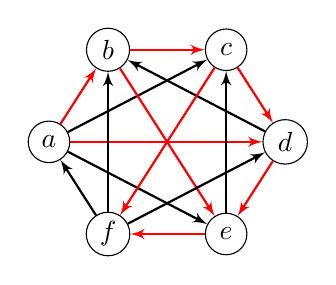
\begin{tikzpicture}
\tikzset{vertex/.style = {shape=circle,draw,minimum size=1.5em}}
\tikzset{edge/.style = {->,> = latex'}}
\node[vertex] (v_0_1) at (-3.0,1.5) {$\!a\!$};
\node[vertex] (v_0_2) at (-2.25,2.67) {$\!b\!$};
\node[vertex] (v_0_3) at (-0.75,2.67) {$\!c\!$};
\node[vertex] (v_0_4) at (-0.0,1.5) {$\!d\!$};
\node[vertex] (v_0_5) at (-0.75,0.33) {$\!e\!$};
\node[vertex] (v_0_6) at (-2.25,0.33) {$\!\!\!f\!\!\!$};
\draw[edge, thick][red] (v_0_1) to (v_0_2);
\draw[edge, thick] (v_0_1) to (v_0_3);
\draw[edge, thick][red] (v_0_2) to (v_0_3);
\draw[edge, thick][red] (v_0_1) to (v_0_4);
\draw[edge, thick] (v_0_4) to (v_0_2);
\draw[edge, thick][red] (v_0_3) to (v_0_4);
\draw[edge, thick] (v_0_1) to (v_0_5);
\draw[edge, thick][red] (v_0_2) to (v_0_5);
\draw[edge, thick] (v_0_5) to (v_0_3);
\draw[edge, thick][red] (v_0_4) to (v_0_5);
\draw[edge, thick] (v_0_6) to (v_0_1);
\draw[edge, thick] (v_0_6) to (v_0_2);
\draw[edge, thick][red] (v_0_3) to (v_0_6);
\draw[edge, thick] (v_0_6) to (v_0_4);
\draw[edge, thick][red] (v_0_5) to (v_0_6);
\end{tikzpicture}

\caption{One of the 56 isomorphism class representatives admitted by a particular isolator for 6-vertex tournaments. Red edges are edges fixed by unit clauses of the isolator.} \label{fig3}
\end{figure}

 For $n = 7$, solving the SAT instance directly became clearly infeasible (taking several days without any signs of progress). However, random probing allowed us to find a perfect isolator for $n=7,8$. Each probe ran in around 10 seconds when restricted to force a positive literal in each clause with the map file reduced by the unit clauses from the next largest isolator.  Table \ref{tab:smallest_isolators_found} describes the best (fewest non-unit clauses) isolator found for $1 \le n \le 8$. Several thousand probes were required to find our best known isolator for $n=7$, while 2 probes were used to find our $n=8$ isolator (each $n=8$ probe required about 2 days to finish). We note that $n=8$ isolators can have up to $11$ unit clauses; the $n=8$ isolator in Table \ref{tab:smallest_isolators_found} was the shortest \emph{perfect} isolator we generated via probing.

\begin{table}[ht]
    \centering
        \caption{Shortest Perfect isolators found for $n\le 8$}
    \begin{tabular}{c|c|c|c}
        Vertices & Isomorphism classes &Best units & Best non-units  \\ \hline
        1&1&0&0\\ 
        2&1&1&0\\ 
        3&2&2&0\\ 
        4&4&4&0\\
        5&12&6&2\\ 
        6&56&8&6\\ 
        7&456&9&47\\ 
        8&6880&10 & 665 \\
    \end{tabular}

    \label{tab:smallest_isolators_found}
\end{table}


\begin{figure}[h]
\centering
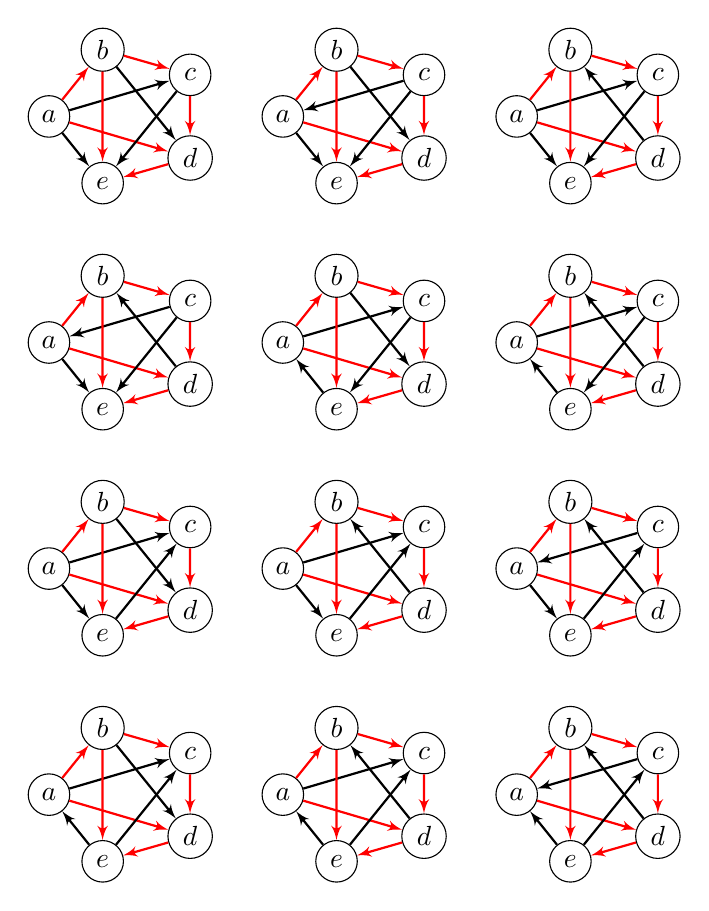
\begin{tikzpicture}[scale=1.1]
\tikzset{vertex/.style = {shape=circle,draw,minimum size=1.5em}}
\tikzset{edge/.style = {->,> = latex'}}
\node[vertex] (v_0_1) at (-1.8,0.9) {$\!a\!$};
\node[vertex] (v_0_2) at (-1.18,1.67) {$\!b\!$};
\node[vertex] (v_0_3) at (-0.17,1.38) {$\!c\!$};
\node[vertex] (v_0_4) at (-0.17,0.42) {$\!d\!$};
\node[vertex] (v_0_5) at (-1.18,0.13) {$\!e\!$};
\draw[edge, thick][red] (v_0_1) to (v_0_2);
\draw[edge, thick] (v_0_3) to (v_0_1);
\draw[edge, thick][red] (v_0_2) to (v_0_3);
\draw[edge, thick][red] (v_0_1) to (v_0_4);
\draw[edge, thick] (v_0_4) to (v_0_2);
\draw[edge, thick][red] (v_0_3) to (v_0_4);
\draw[edge, thick] (v_0_5) to (v_0_1);
\draw[edge, thick][red] (v_0_2) to (v_0_5);
\draw[edge, thick] (v_0_5) to (v_0_3);
\draw[edge, thick][red] (v_0_4) to (v_0_5);
\node[vertex] (v_1_1) at (-4.5,0.9) {$\!a\!$};
\node[vertex] (v_1_2) at (-3.88,1.67) {$\!b\!$};
\node[vertex] (v_1_3) at (-2.87,1.38) {$\!c\!$};
\node[vertex] (v_1_4) at (-2.87,0.42) {$\!d\!$};
\node[vertex] (v_1_5) at (-3.88,0.13) {$\!e\!$};
\draw[edge, thick][red] (v_1_1) to (v_1_2);
\draw[edge, thick] (v_1_1) to (v_1_3);
\draw[edge, thick][red] (v_1_2) to (v_1_3);
\draw[edge, thick][red] (v_1_1) to (v_1_4);
\draw[edge, thick] (v_1_4) to (v_1_2);
\draw[edge, thick][red] (v_1_3) to (v_1_4);
\draw[edge, thick] (v_1_5) to (v_1_1);
\draw[edge, thick][red] (v_1_2) to (v_1_5);
\draw[edge, thick] (v_1_5) to (v_1_3);
\draw[edge, thick][red] (v_1_4) to (v_1_5);
\node[vertex] (v_2_1) at (-7.2,0.9) {$\!a\!$};
\node[vertex] (v_2_2) at (-6.58,1.67) {$\!b\!$};
\node[vertex] (v_2_3) at (-5.57,1.38) {$\!c\!$};
\node[vertex] (v_2_4) at (-5.57,0.42) {$\!d\!$};
\node[vertex] (v_2_5) at (-6.58,0.13) {$\!e\!$};
\draw[edge, thick][red] (v_2_1) to (v_2_2);
\draw[edge, thick] (v_2_1) to (v_2_3);
\draw[edge, thick][red] (v_2_2) to (v_2_3);
\draw[edge, thick][red] (v_2_1) to (v_2_4);
\draw[edge, thick] (v_2_2) to (v_2_4);
\draw[edge, thick][red] (v_2_3) to (v_2_4);
\draw[edge, thick] (v_2_5) to (v_2_1);
\draw[edge, thick][red] (v_2_2) to (v_2_5);
\draw[edge, thick] (v_2_5) to (v_2_3);
\draw[edge, thick][red] (v_2_4) to (v_2_5);
\node[vertex] (v_3_1) at (-1.8,3.51) {$\!a\!$};
\node[vertex] (v_3_2) at (-1.18,4.28) {$\!b\!$};
\node[vertex] (v_3_3) at (-0.17,3.99) {$\!c\!$};
\node[vertex] (v_3_4) at (-0.17,3.03) {$\!d\!$};
\node[vertex] (v_3_5) at (-1.18,2.74) {$\!e\!$};
\draw[edge, thick][red] (v_3_1) to (v_3_2);
\draw[edge, thick] (v_3_3) to (v_3_1);
\draw[edge, thick][red] (v_3_2) to (v_3_3);
\draw[edge, thick][red] (v_3_1) to (v_3_4);
\draw[edge, thick] (v_3_4) to (v_3_2);
\draw[edge, thick][red] (v_3_3) to (v_3_4);
\draw[edge, thick] (v_3_1) to (v_3_5);
\draw[edge, thick][red] (v_3_2) to (v_3_5);
\draw[edge, thick] (v_3_5) to (v_3_3);
\draw[edge, thick][red] (v_3_4) to (v_3_5);
\node[vertex] (v_4_1) at (-4.5,3.51) {$\!a\!$};
\node[vertex] (v_4_2) at (-3.88,4.28) {$\!b\!$};
\node[vertex] (v_4_3) at (-2.87,3.99) {$\!c\!$};
\node[vertex] (v_4_4) at (-2.87,3.03) {$\!d\!$};
\node[vertex] (v_4_5) at (-3.88,2.74) {$\!e\!$};
\draw[edge, thick][red] (v_4_1) to (v_4_2);
\draw[edge, thick] (v_4_1) to (v_4_3);
\draw[edge, thick][red] (v_4_2) to (v_4_3);
\draw[edge, thick][red] (v_4_1) to (v_4_4);
\draw[edge, thick] (v_4_4) to (v_4_2);
\draw[edge, thick][red] (v_4_3) to (v_4_4);
\draw[edge, thick] (v_4_1) to (v_4_5);
\draw[edge, thick][red] (v_4_2) to (v_4_5);
\draw[edge, thick] (v_4_5) to (v_4_3);
\draw[edge, thick][red] (v_4_4) to (v_4_5);
\node[vertex] (v_5_1) at (-7.2,3.51) {$\!a\!$};
\node[vertex] (v_5_2) at (-6.58,4.28) {$\!b\!$};
\node[vertex] (v_5_3) at (-5.57,3.99) {$\!c\!$};
\node[vertex] (v_5_4) at (-5.57,3.03) {$\!d\!$};
\node[vertex] (v_5_5) at (-6.58,2.74) {$\!e\!$};
\draw[edge, thick][red] (v_5_1) to (v_5_2);
\draw[edge, thick] (v_5_1) to (v_5_3);
\draw[edge, thick][red] (v_5_2) to (v_5_3);
\draw[edge, thick][red] (v_5_1) to (v_5_4);
\draw[edge, thick] (v_5_2) to (v_5_4);
\draw[edge, thick][red] (v_5_3) to (v_5_4);
\draw[edge, thick] (v_5_1) to (v_5_5);
\draw[edge, thick][red] (v_5_2) to (v_5_5);
\draw[edge, thick] (v_5_5) to (v_5_3);
\draw[edge, thick][red] (v_5_4) to (v_5_5);
\node[vertex] (v_6_1) at (-1.8,6.12) {$\!a\!$};
\node[vertex] (v_6_2) at (-1.18,6.89) {$\!b\!$};
\node[vertex] (v_6_3) at (-0.17,6.6) {$\!c\!$};
\node[vertex] (v_6_4) at (-0.17,5.64) {$\!d\!$};
\node[vertex] (v_6_5) at (-1.18,5.35) {$\!e\!$};
\draw[edge, thick][red] (v_6_1) to (v_6_2);
\draw[edge, thick] (v_6_1) to (v_6_3);
\draw[edge, thick][red] (v_6_2) to (v_6_3);
\draw[edge, thick][red] (v_6_1) to (v_6_4);
\draw[edge, thick] (v_6_4) to (v_6_2);
\draw[edge, thick][red] (v_6_3) to (v_6_4);
\draw[edge, thick] (v_6_5) to (v_6_1);
\draw[edge, thick][red] (v_6_2) to (v_6_5);
\draw[edge, thick] (v_6_3) to (v_6_5);
\draw[edge, thick][red] (v_6_4) to (v_6_5);
\node[vertex] (v_7_1) at (-4.5,6.12) {$\!a\!$};
\node[vertex] (v_7_2) at (-3.88,6.89) {$\!b\!$};
\node[vertex] (v_7_3) at (-2.87,6.6) {$\!c\!$};
\node[vertex] (v_7_4) at (-2.87,5.64) {$\!d\!$};
\node[vertex] (v_7_5) at (-3.88,5.35) {$\!e\!$};
\draw[edge, thick][red] (v_7_1) to (v_7_2);
\draw[edge, thick] (v_7_1) to (v_7_3);
\draw[edge, thick][red] (v_7_2) to (v_7_3);
\draw[edge, thick][red] (v_7_1) to (v_7_4);
\draw[edge, thick] (v_7_2) to (v_7_4);
\draw[edge, thick][red] (v_7_3) to (v_7_4);
\draw[edge, thick] (v_7_5) to (v_7_1);
\draw[edge, thick][red] (v_7_2) to (v_7_5);
\draw[edge, thick] (v_7_3) to (v_7_5);
\draw[edge, thick][red] (v_7_4) to (v_7_5);
\node[vertex] (v_8_1) at (-7.2,6.12) {$\!a\!$};
\node[vertex] (v_8_2) at (-6.58,6.89) {$\!b\!$};
\node[vertex] (v_8_3) at (-5.57,6.6) {$\!c\!$};
\node[vertex] (v_8_4) at (-5.57,5.64) {$\!d\!$};
\node[vertex] (v_8_5) at (-6.58,5.35) {$\!e\!$};
\draw[edge, thick][red] (v_8_1) to (v_8_2);
\draw[edge, thick] (v_8_3) to (v_8_1);
\draw[edge, thick][red] (v_8_2) to (v_8_3);
\draw[edge, thick][red] (v_8_1) to (v_8_4);
\draw[edge, thick] (v_8_4) to (v_8_2);
\draw[edge, thick][red] (v_8_3) to (v_8_4);
\draw[edge, thick] (v_8_1) to (v_8_5);
\draw[edge, thick][red] (v_8_2) to (v_8_5);
\draw[edge, thick] (v_8_3) to (v_8_5);
\draw[edge, thick][red] (v_8_4) to (v_8_5);
\node[vertex] (v_9_1) at (-1.8,8.73) {$\!a\!$};
\node[vertex] (v_9_2) at (-1.18,9.5) {$\!b\!$};
\node[vertex] (v_9_3) at (-0.17,9.21) {$\!c\!$};
\node[vertex] (v_9_4) at (-0.17,8.25) {$\!d\!$};
\node[vertex] (v_9_5) at (-1.18,7.96) {$\!e\!$};
\draw[edge, thick][red] (v_9_1) to (v_9_2);
\draw[edge, thick] (v_9_1) to (v_9_3);
\draw[edge, thick][red] (v_9_2) to (v_9_3);
\draw[edge, thick][red] (v_9_1) to (v_9_4);
\draw[edge, thick] (v_9_4) to (v_9_2);
\draw[edge, thick][red] (v_9_3) to (v_9_4);
\draw[edge, thick] (v_9_1) to (v_9_5);
\draw[edge, thick][red] (v_9_2) to (v_9_5);
\draw[edge, thick] (v_9_3) to (v_9_5);
\draw[edge, thick][red] (v_9_4) to (v_9_5);
\node[vertex] (v_10_1) at (-4.5,8.73) {$\!a\!$};
\node[vertex] (v_10_2) at (-3.88,9.5) {$\!b\!$};
\node[vertex] (v_10_3) at (-2.87,9.21) {$\!c\!$};
\node[vertex] (v_10_4) at (-2.87,8.25) {$\!d\!$};
\node[vertex] (v_10_5) at (-3.88,7.96) {$\!e\!$};
\draw[edge, thick][red] (v_10_1) to (v_10_2);
\draw[edge, thick] (v_10_3) to (v_10_1);
\draw[edge, thick][red] (v_10_2) to (v_10_3);
\draw[edge, thick][red] (v_10_1) to (v_10_4);
\draw[edge, thick] (v_10_2) to (v_10_4);
\draw[edge, thick][red] (v_10_3) to (v_10_4);
\draw[edge, thick] (v_10_1) to (v_10_5);
\draw[edge, thick][red] (v_10_2) to (v_10_5);
\draw[edge, thick] (v_10_3) to (v_10_5);
\draw[edge, thick][red] (v_10_4) to (v_10_5);
\node[vertex] (v_11_1) at (-7.2,8.73) {$\!a\!$};
\node[vertex] (v_11_2) at (-6.58,9.5) {$\!b\!$};
\node[vertex] (v_11_3) at (-5.57,9.21) {$\!c\!$};
\node[vertex] (v_11_4) at (-5.57,8.25) {$\!d\!$};
\node[vertex] (v_11_5) at (-6.58,7.96) {$\!e\!$};
\draw[edge, thick][red] (v_11_1) to (v_11_2);
\draw[edge, thick] (v_11_1) to (v_11_3);
\draw[edge, thick][red] (v_11_2) to (v_11_3);
\draw[edge, thick][red] (v_11_1) to (v_11_4);
\draw[edge, thick] (v_11_2) to (v_11_4);
\draw[edge, thick][red] (v_11_3) to (v_11_4);
\draw[edge, thick] (v_11_1) to (v_11_5);
\draw[edge, thick][red] (v_11_2) to (v_11_5);
\draw[edge, thick] (v_11_3) to (v_11_5);
\draw[edge, thick][red] (v_11_4) to (v_11_5);
\end{tikzpicture}

\caption{All isomorphism class representatives admitted by a particular isolator for 5-vertex tournaments. Red edges are edges fixed by unit clauses of the isolator. The two non-unit clauses in the isolator are $ac \lor \lnot bd \lor ce$ and $ac \lor ae \lor \lnot ce$.} \label{fig2}
\end{figure}

\subsection{Tournament Ramsey Graphs}

The known tournament Ramsey numbers are $R(2) = 2$, $R(3) = 4$, $R(4) = 8$, $R(5) = 14$, and $R(6) = 28$~\cite{SanchezFlores54}. 
Note that in most cases, the next number is two times it predecessor.
Recently, the lower and upper bounds for $R(7)$ have been improved from $32 \leq R(7) \leq 54$ to $34 \leq R(7) \leq 47$~\cite{directedramsey}. 
The improved lower bound is due to dozens of $TT_7$-free tournament on 33-vertices found using SAT. 

McKay~\cite{McKay} extended this set of 33-vertex $TT_7$-free tournaments to 5303 using the following method: generate all 29-vertex subtournaments of known 33-vertex $TT_7$-free tournaments and extend them in all possible ways to 33-vertex $TT_7$-free tournaments. Repeat this procedure until no new 33-vertex $TT_7$-free tournaments are found. Also note that if a tournament has no $TT_k$, then its complement (reversing all arcs) also doesn't. This can be used to find additional $TT_k$-free graphs as well. 

Looking for neighbors and complement graphs is a well-known technique to compute more graphs with a certain property. McKay and Radziszowski used it to compute all known 42-vertex graphs that have no clique of size 5 nor a co-clique of size 5~\cite{McKay1997}. They conjecture that this method generated all possible graphs of this type. 

For all known Ramsey numbers $R(k)$, there are unique tournaments without a $TT_k$ of size $R(k)-1$ and $R(k)-2$. Generalizing this property, if for some $n$ there exists a $k$ with a unique $TT_k$-free tournament on $n$ vertices, then that graph is known as $\mathit{ST}_n$. For example, the unique $TT_6$-free tournaments on $26$ and $27$ vertices are referred to as $\mathit{ST}_{26}$ and $\mathit{ST}_{27}$ respectively. 

Prior to our work, there were 5303 known $TT_7$-free tournaments on $33$ vertices, implying that $R(7) \geq 34$. So, either $k=7$ breaks the pattern of existence of $\mathit{ST}_n$ tournaments, or $R(7) > 34$. 
 We studied the 5303 33-vertex $TT_7$-free tournaments and
found that all of them have $\mathit{ST}_{26}$ as a subtournament. Moreover, 4952 of them have $\mathit{ST}_{27}$ as a subtournament. 



It is the case that any $TT_7$-free tournament on $34$ vertices contains at least 1 (up to isomorphism) $TT_7$-free subtournament on $33$ vertices. Therefore, enumerating further $TT_7$-free tournaments on 33 vertices is a step towards either finding a $TT_7$-free 34-vertex tournament or proving that no such tournament exists. With this motivation, we explored whether the suite of 5303 was complete or whether there are any other 33-vertex $TT_7$-free tournaments.
 Our main experimental setup involved finding new members containing $\mathit{ST}_{26}$ but not $\mathit{ST}_{27}$ by solving a CNF formula with a SAT solver, which uses our isolator on 7 vertices. The formula can be described as the union of the following sets of clauses:
 
 \begin{enumerate}
 \item ${26 \choose 2} = 325$ unit clauses requiring that $\mathit{ST}_{26}$ be present in vertices $v_1$ through $v_{26}$;
 \item The perfect isolator for $n=7$ on the seven remaining vertices $v_{27}$ through $v_{33}$;
 \item A clause blocking each of the 5303 known solutions for each vertex permutation that caused the solution to have $\mathit{ST}_{26}$ in vertices $v_1$ through $v_{26}$ and a graph admitted by the $n=7$ isolator in vertices $v_{27}$ through $v_{33}$; and
 \item clauses enforcing the ``no $TT_7$'' condition from \cite{directedramsey}.
 \end{enumerate}

While this formula does not disallow all $\mathit{ST}_{27}$s (i.e. a solution might include an extension from $\mathit{ST}_{26}$ that was not present in the original solution set), it disallows all currently known extensions, including the most common by far $1$-vertex extension from $\mathit{ST}_{26}$ to $\mathit{ST}_{27}$. Additionally, the $n=7$ perfect isolator plays a crucial role for finding new solutions in that without it, the SAT solver could find any tournament equivalent to one of the previously known 33-vertex $TT_7$-free tournaments  except for some non-automorphic permutation of the last 7 vertices (which would thus be isomorphic to the previously known solution). We claim that all solutions to our formula must be non-isomorphic to the original 5303 tournaments. 

On the Pittsburgh Supercomputing Center~\cite{cluster}, we ran 640 shuffled (clause permuted) versions of the above formula on 640 cores for 6 hours using the Kissat solver~\cite{Kissat}. We found three different satisfying assignments. These three solutions represented  a single new 33-vertex $TT_7$-free tournament, which is shown in Figure~\ref{newtournament} in the appendix. This tournament is special as it is self-complementary: reversing all arcs result in an isomorphic graph. Only a small fraction of tournaments has this self-complementary property~\cite{Eplett}. Note that all $\mathit{ST}_n$ graphs have this property by definition. After finding this new tournament, we updated the formula to include the blocking clauses for the new tournaments and its isomorphisms. Kissat did not produce further solutions when using 640 shuffled (clause permuted) version of the updated formula on 640 cores in a day, so it is possible that the formula is simply unsatisfiable. 


\section{Conclusions}

Our techniques allow the generation of isolators with asymptotically optimal numbers of unit clauses, as well as perfect, optimal isolators for $n \le 6$ and compact isolators for $n=7,8$ found by random probing. We further demonstrate how small isolators can be effectively used in the search for much larger graphs relevant to tournament existence problems. Future work using our results may lead to further improvements on bounds for the tournament Ramsey number problem.

\section*{Acknowledgements}

This work was partially supported by the Hoskinson Center for Formal Mathematics and the National Science Foundation under grant CCF-2015445. We thank Jeremy Avigad for his comments on earlier drafts and John Mackey for his advice on the graph theoretical parts of the paper. 


\clearpage

\bibliographystyle{IEEEtran}
\bibliography{main}
\clearpage
\appendix
\begin{figure}[h!]
$$\left[
\begin{array}{c@{\,}c@{\,}c@{\,}c@{\,}c@{\,}c@{\,}c@{\,}c@{\,}c@{\,}c@{\,}c@{\,}c@{\,}c@{\,}c@{\,}c@{\,}c@{\,}c@{\,}c@{\,}c@{\,}c@{\,}c@{\,}c@{\,}c@{\,}c@{\,}c@{\,}c@{\,}|c@{\,}c@{\,}c@{\,}c@{\,}c@{\,}c@{\,}c}
\zero & \one & \one & \one & \one & \zero & \one & \zero & \zero & \one & \one & \zero & \one & \one & \zero & \zero & \zero & \one & \one & \zero & \zero & \zero & \zero & \one & \zero & \one & \one & \zero & \zero & \one & \one & \zero & \zero \\
\zero & \zero & \zero & \zero & \zero & \zero & \one & \zero & \one & \one & \zero & \zero & \one & \zero & \zero & \one & \one & \one & \zero & \zero & \one & \one & \one & \one & \zero & \one & \one & \zero & \zero & \one & \one & \zero & \one \\
\zero & \one & \zero & \one & \one & \one & \one & \zero & \one & \zero & \zero & \one & \one & \zero & \one & \one & \zero & \zero & \zero & \one & \one & \zero & \zero & \zero & \zero & \one & \zero & \zero & \zero & \zero & \zero & \zero & \one \\
\zero & \one & \zero & \zero & \zero & \zero & \zero & \zero & \one & \zero & \one & \one & \zero & \zero & \one & \zero & \zero & \one & \one & \one & \zero & \zero & \one & \one & \one & \one & \one & \zero & \one & \zero & \one & \zero & \one \\
\zero & \one & \zero & \one & \zero & \one & \one & \one & \one & \zero & \one & \zero & \zero & \one & \one & \zero & \one & \one & \zero & \zero & \zero & \one & \one & \zero & \zero & \zero & \one & \zero & \one & \zero & \zero & \one & \zero \\
\one & \one & \zero & \one & \zero & \zero & \zero & \zero & \zero & \zero & \one & \zero & \one & \one & \zero & \zero & \one & \zero & \zero & \one & \one & \one & \zero & \zero & \one & \one & \zero & \one & \one & \zero & \zero & \one & \one \\
\zero & \zero & \zero & \one & \zero & \one & \zero & \one & \one & \one & \one & \zero & \one & \zero & \zero & \one & \one & \zero & \one & \one & \zero & \zero & \zero & \one & \one & \zero & \zero & \zero & \one & \one & \one & \zero & \zero \\
\one & \one & \one & \one & \zero & \one & \zero & \zero & \zero & \zero & \zero & \zero & \one & \zero & \one & \one & \zero & \zero & \one & \zero & \zero & \one & \one & \one & \zero & \zero & \one & \one & \zero & \zero & \one & \zero & \one \\
\one & \zero & \zero & \zero & \zero & \one & \zero & \one & \zero & \one & \one & \one & \one & \zero & \one & \zero & \zero & \one & \one & \zero & \one & \one & \zero & \zero & \zero & \one & \zero & \one & \one & \one & \zero & \zero & \zero \\
\zero & \zero & \one & \one & \one & \one & \zero & \one & \zero & \zero & \zero & \zero & \zero & \zero & \one & \zero & \one & \one & \zero & \zero & \one & \zero & \zero & \one & \one & \one & \one & \one & \one & \zero & \zero & \one & \zero \\
\zero & \one & \one & \zero & \zero & \zero & \zero & \one & \zero & \one & \zero & \one & \one & \one & \one & \zero & \one & \zero & \zero & \one & \one & \zero & \one & \one & \zero & \zero & \zero & \one & \zero & \one & \zero & \one & \zero \\
\one & \one & \zero & \zero & \one & \one & \one & \one & \zero & \one & \zero & \zero & \zero & \zero & \zero & \zero & \one & \zero & \one & \one & \zero & \zero & \one & \zero & \zero & \one & \one & \one & \zero & \one & \zero & \zero & \one \\
\zero & \zero & \zero & \one & \one & \zero & \zero & \zero & \zero & \one & \zero & \one & \zero & \one & \one & \one & \one & \zero & \one & \zero & \zero & \one & \one & \zero & \one & \one & \one & \zero & \zero & \one & \zero & \one & \zero \\
\zero & \one & \one & \one & \zero & \zero & \one & \one & \one & \one & \zero & \one & \zero & \zero & \zero & \zero & \zero & \zero & \one & \zero & \one & \one & \zero & \zero & \one & \zero & \one & \one & \one & \zero & \one & \zero & \zero \\
\one & \one & \zero & \zero & \zero & \one & \one & \zero & \zero & \zero & \zero & \one & \zero & \one & \zero & \one & \one & \one & \one & \zero & \one & \zero & \zero & \one & \one & \zero & \zero & \one & \zero & \zero & \one & \one & \zero \\
\one & \zero & \zero & \one & \one & \one & \zero & \zero & \one & \one & \one & \one & \zero & \one & \zero & \zero & \zero & \zero & \zero & \zero & \one & \zero & \one & \one & \zero & \zero & \one & \one & \one & \one & \one & \one & \zero \\
\one & \zero & \one & \one & \zero & \zero & \zero & \one & \one & \zero & \zero & \zero & \zero & \one & \zero & \one & \zero & \one & \one & \one & \one & \zero & \one & \zero & \zero & \one & \one & \one & \zero & \zero & \zero & \one & \zero \\
\zero & \zero & \one & \zero & \zero & \one & \one & \one & \zero & \zero & \one & \one & \one & \one & \zero & \one & \zero & \zero & \zero & \zero & \zero & \zero & \one & \zero & \one & \one & \one & \zero & \one & \zero & \zero & \one & \one \\
\zero & \one & \one & \zero & \one & \one & \zero & \zero & \zero & \one & \one & \zero & \zero & \zero & \zero & \one & \zero & \one & \zero & \one & \one & \one & \one & \zero & \one & \zero & \one & \zero & \one & \one & \zero & \zero & \zero \\
\one & \one & \zero & \zero & \one & \zero & \zero & \one & \one & \one & \zero & \zero & \one & \one & \one & \one & \zero & \one & \zero & \zero & \zero & \zero & \zero & \zero & \one & \zero & \zero & \one & \zero & \one & \zero & \one & \one \\
\one & \zero & \zero & \one & \one & \zero & \one & \one & \zero & \zero & \zero & \one & \one & \zero & \zero & \zero & \zero & \one & \zero & \one & \zero & \one & \one & \one & \one & \zero & \one & \one & \zero & \zero & \one & \zero & \zero \\
\one & \zero & \one & \one & \zero & \zero & \one & \zero & \zero & \one & \one & \one & \zero & \zero & \one & \one & \one & \one & \zero & \one & \zero & \zero & \zero & \zero & \zero & \zero & \zero & \one & \one & \one & \zero & \zero & \one \\
\one & \zero & \one & \zero & \zero & \one & \one & \zero & \one & \one & \zero & \zero & \zero & \one & \one & \zero & \zero & \zero & \zero & \one & \zero & \one & \zero & \one & \one & \one & \zero & \zero & \one & \zero & \one & \one & \zero \\
\zero & \zero & \one & \zero & \one & \one & \zero & \zero & \one & \zero & \zero & \one & \one & \one & \zero & \zero & \one & \one & \one & \one & \zero & \one & \zero & \zero & \zero & \zero & \one & \one & \one & \one & \zero & \zero & \zero \\
\one & \one & \one & \zero & \one & \zero & \zero & \one & \one & \zero & \one & \one & \zero & \zero & \zero & \one & \one & \zero & \zero & \zero & \zero & \one & \zero & \one & \zero & \one & \zero & \one & \one & \zero & \one & \zero & \zero \\
\zero & \zero & \zero & \zero & \one & \zero & \one & \one & \zero & \zero & \one & \zero & \zero & \one & \one & \one & \zero & \zero & \one & \one & \one & \one & \zero & \one & \zero & \zero & \zero & \zero & \one & \zero & \one & \one & \one \\
  \hline
\zero & \zero & \one & \zero & \zero & \one & \one & \zero & \one & \zero & \one & \zero & \zero & \zero & \one & \zero & \zero & \zero & \zero & \one & \zero & \one & \one & \zero & \one & \one & \zero & \one & \zero & \one & \one & \one & \one \\
\one & \one & \one & \one & \one & \zero & \one & \zero & \zero & \zero & \zero & \zero & \one & \zero & \zero & \zero & \zero & \one & \one & \zero & \zero & \zero & \one & \zero & \zero & \one & \zero & \zero & \one & \one & \one & \one & \one \\
\one & \one & \one & \zero & \zero & \zero & \zero & \one & \zero & \zero & \one & \one & \one & \zero & \one & \zero & \one & \zero & \zero & \one & \one & \zero & \zero & \zero & \zero & \zero & \one & \zero & \zero & \one & \one & \one & \one \\
\zero & \zero & \one & \one & \one & \one & \zero & \one & \zero & \one & \zero & \zero & \zero & \one & \one & \zero & \one & \one & \zero & \zero & \one & \zero & \one & \zero & \one & \one & \zero & \zero & \zero & \zero & \one & \zero & \one \\
\zero & \zero & \one & \zero & \one & \one & \zero & \zero & \one & \one & \one & \one & \one & \zero & \zero & \zero & \one & \one & \one & \one & \zero & \one & \zero & \one & \zero & \zero & \zero & \zero & \zero & \zero & \zero & \one & \one \\
\one & \one & \one & \one & \zero & \zero & \one & \one & \one & \zero & \zero & \one & \zero & \one & \zero & \zero & \zero & \zero & \one & \zero & \one & \one & \zero & \one & \one & \zero & \zero & \zero & \zero & \one & \zero & \zero & \one \\
\one & \zero & \zero & \zero & \one & \zero & \one & \zero & \one & \one & \one & \zero & \one & \one & \one & \one & \one & \zero & \one & \zero & \one & \zero & \one & \one & \one & \zero & \zero & \zero & \zero & \zero & \zero & \zero & \zero \\
\end{array}
\right]$$

\caption{The new 33-vertex $TT_7$-free tournament found using our perfect isolator for $n=7$. The upper-left section of the matrix is $\mathit{ST}_{26}$, while the bottom-right section is a graph admitted by our $n=7$ isolator.}
\label{newtournament}
\end{figure}

\end{document}
